\documentclass[11pt]{article}

% ---------------------------------------------------------------------------
% ISAN 3392 research proposal: Predictive GPU Right-Sizing
% Build:  tectonic main.tex      (figures: python scripts/make_figures.py)
% This is the long "research-trail" version. Do not compress yet.
% ---------------------------------------------------------------------------

\usepackage[margin=1in]{geometry}
\usepackage[T1]{fontenc}
\usepackage{lmodern}
\usepackage{microtype}
\usepackage{amsmath,amssymb}
\usepackage{graphicx}
\usepackage{booktabs}
\usepackage{tabularx}
\usepackage{array}
\usepackage{longtable}
\usepackage{multirow}
\usepackage[table]{xcolor}
\usepackage{enumitem}
\usepackage{caption}
\usepackage{subcaption}
\usepackage{tikz}
\usetikzlibrary{arrows.meta,positioning,shapes.geometric,fit,calc}
\usepackage{pgfgantt}
\usepackage{tcolorbox}
\usepackage[numbers,sort&compress]{natbib}
\usepackage[colorlinks=true,linkcolor=blue!50!black,citecolor=blue!50!black,urlcolor=blue!50!black]{hyperref}
\usepackage{cleveref}
\usepackage{xurl}
\usepackage{makecell}

\definecolor{accent}{HTML}{2a78d6}
\definecolor{good}{HTML}{1baf7a}
\definecolor{warn}{HTML}{eb6834}
\definecolor{soft}{HTML}{f3f2ee}

\newcolumntype{L}{>{\raggedright\arraybackslash}X}
\newcolumntype{P}[1]{>{\raggedright\arraybackslash}p{#1}}
\usepackage{float}
\newcommand{\ra}{$\rightarrow$}
\newcommand{\status}[1]{\textsc{#1}}

\newtcolorbox{keybox}[1][]{colback=soft,colframe=accent,boxrule=0.6pt,arc=2pt,left=6pt,right=6pt,top=4pt,bottom=4pt,title={#1},fonttitle=\bfseries\small,coltitle=white}

\captionsetup{font=small,labelfont=bf}
\setlist{itemsep=2pt,topsep=3pt}

\title{\textbf{Predictive GPU Right-Sizing for Production Online Inference}\\[4pt]
\large A Research Proposal Grounded in the Alibaba Serverless Infrastructure GPU Trace}
\author{Saksham Adhikari \and Sudip Bhandari\\[4pt]
\normalsize Advisor: Dr.\ Fred Zhao\\[2pt]
\normalsize ISAN 3392 \textbullet{} Texas State University}
\date{Fall 2026 \textbullet{} Working draft, \today}

\begin{document}
\maketitle

\begin{abstract}
\noindent Production GPU fleets serving online inference are routinely over-reserved: operators trade utilization for latency headroom because an under-provisioned inference pod hurts users directly. We ask how much of that reserved capacity can be recovered by predicting, at admission, the smallest safe GPU slice a pod needs (\emph{Model A, allocation}), and what placement risk the recovery carries (\emph{Model B, readiness/failure}). Using the six-month Alibaba Serverless Infrastructure (ASI) trace released with OSDI~'26 (up to 155{,}410 GPUs on 37{,}707 servers), we built two datasets (294{,}465 pods for right-sizing; 2{,}826{,}036 pods for placement) and evaluated history-rule, linear, and gradient-boosted models under a pre-registered go/no-go gate on ten held-out clusters. At a fixed 5\% under-provisioning budget, roughly \textbf{21--25\% of reserved online-inference GPU-hours} are reclaimable on clusters never seen in training, almost entirely from recommendation pods with workload history; GenAI pods have a median minimum viable fraction of 0.983 of a GPU, consistent with ASI's report that GenAI inference fills GPU memory while leaving compute mostly idle. A simple workload-history rule captures nearly all of it (20.8\% vs.\ 21.9\% for XGBoost), so the learned model returned \textsc{no-go} on its accuracy gate. Model B predicts failure to become ready with ROC-AUC 0.75 in known clusters but 0.65 and poorly calibrated on unseen clusters. This document preserves the full research trail (hypotheses, experiments, failures, and comparisons), positions the results against commercial GPU schedulers at Google, AWS, Microsoft, NVIDIA, Meta, and Alibaba itself, quantifies business value, and proposes the next round of experiments: workload-mixing signals (recommendation vs.\ GenAI co-location), workload--GPU compatibility, production vs.\ non-production behaviour, runtime patterns, and explicit safety constraints.
\end{abstract}

\begin{keybox}[Reading guide]
\small
\begin{tabularx}{\linewidth}{@{}lL@{}}
\textbf{Model A} & \emph{Allocation.} Predicts the minimum viable GPU fraction (MVF) per online-inference pod at admission, with a conformal safety margin. Success = reserved GPU-hours reclaimed ($R$) at under-provisioning rate $U \le 5\%$. \\
\textbf{Model B} & \emph{Readiness/failure.} Predicts the probability a pod fails to become ready when placed. Success = discrimination (ROC/PR-AUC) and calibration (ECE) that hold on unseen clusters. \\
\textbf{Status tags} & \status{done} = run and reported; \status{proposed} = designed here, not yet run. No numbers in this document are reported for \status{proposed} experiments. \\
\end{tabularx}
\end{keybox}

\tableofcontents
\newpage

% ===========================================================================
\section{Motivation and Problem Statement}
\label{sec:motivation}

Companies serving interactive AI products (feeds, ads, search ranking, chat assistants) prioritize low tail latency because it drives engagement and satisfaction. The standard operational response is to over-reserve: give each inference pod a whole GPU, or more, and accept low utilization as the price of headroom. Because accelerators dominate the capital and energy cost of an AI datacenter, even small utilization gains translate into large savings.

\paragraph{The utilization identity.} Suppose a fleet of $N$ servers runs at utilization $R_1$, and better allocation raises it to $R_2$ while serving the same work. Ignoring packing and failure constraints, the number of servers $X$ that can be freed satisfies
\begin{equation}
N R_1 = (N - X) R_2 \quad\Longrightarrow\quad X = N\,\frac{R_2 - R_1}{R_2}.
\label{eq:util}
\end{equation}
With $N = 100{,}000$, $R_1 = 28\%$, $R_2 = 40\%$, we obtain $X = 30{,}000$ servers; at an assumed \$5{,}000 per server this is \$150M of avoided capital. \Cref{fig:util} shows the identity is concave: the first points of utilization are the most valuable.

\begin{figure}[h]
\centering
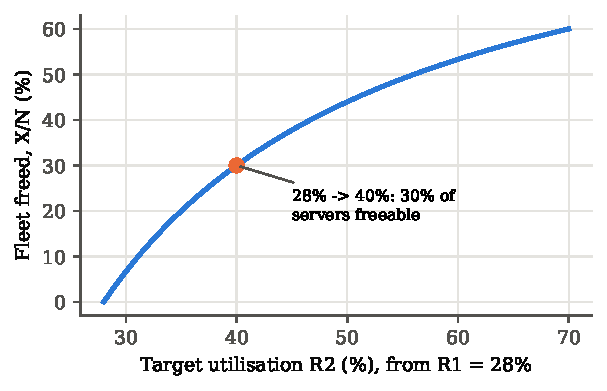
\includegraphics[width=0.55\linewidth]{figures/fig_util.pdf}
\caption{Share of the fleet freed by raising utilization from 28\% to $R_2$ (\cref{eq:util}). Idealized: assumes perfect packing and no added failure risk. Sections~\ref{sec:results} and~\ref{sec:value} show why the realizable number is smaller.}
\label{fig:util}
\end{figure}

\paragraph{Research question.} \emph{How much GPU capacity in production online-inference fleets can be recovered by predicting, at admission, the smallest safe GPU slice a pod needs, and what placement risk does that recovery carry?} We separate the problem into two models with distinct jobs:

\begin{itemize}
  \item \textbf{Model A (allocation / right-sizing):} a quantile regressor for the pod's minimum viable GPU fraction, wrapped in a split-conformal margin so that at most $\approx$5\% of pods are under-provisioned.
  \item \textbf{Model B (readiness / failure):} a calibrated classifier for whether the pod becomes ready after placement, used to veto shrinks that make placement unsafe.
\end{itemize}
Keeping these separate matters: Model A answers ``how much does this pod need?''; Model B answers ``if we give it that, will it come up?'' Conflating them hides the second risk behind the first.

% ===========================================================================
\section{Research Questions and Hypotheses}
\label{sec:rq}

\begin{table}[h]
\centering\small
\caption{Research questions, hypotheses, and current status. H1--H4 were pre-registered before modelling; H5--H10 are added in this proposal.}
\label{tab:hyp}
\begin{tabularx}{\linewidth}{@{}p{0.6cm}Lp{2.2cm}p{2.3cm}@{}}
\toprule
ID & Hypothesis & Model & Status \\
\midrule
H1 & A learned quantile model (A3) predicts minimum viable slice more accurately than a per-workload P90 history rule (A1) on unseen clusters. & A & \status{done}: rejected \\
H2 & Failure to become ready is predictable and calibrated from admission-time features. & B & \status{done}: partly supported \\
H3 & A material share ($>$10\%) of reserved GPU-hours is reclaimable at $U \le 5\%$. & A & \status{done}: supported ($\approx$21\%) \\
H4 & Relationships transfer to clusters unseen in training. & A, B & \status{done}: partly \\
\midrule
H5 & \emph{Workload mixing.} Pods on servers dominated by recommendation workloads have lower, more predictable MVF than pods co-located with GenAI; co-location share improves A's pinball loss and B's PR-AUC. & A, B & \status{proposed} \\
H6 & \emph{Compatibility.} Readiness failure depends on the (workload type $\times$ GPU type $\times$ slice size) interaction, not on each factor alone. & B & \status{proposed} \\
H7 & \emph{Production vs.\ non-production.} High-priority (production) pods have tighter, more stable demand and lower reclaimable share but lower failure; mixing them with low-priority pods raises B's risk for the latter. & A, B & \status{proposed} \\
H8 & \emph{Runtime patterns.} Diurnal amplitude and burstiness from early-life telemetry predict MVF better than static request features for cold-start pods. & A & \status{proposed} \\
H9 & \emph{Safety constraints.} A per-segment risk budget (tighter for GenAI/production, looser for rec/non-production) reclaims more than a uniform 5\% budget at equal expected harm. & A+B & \status{proposed} \\
H10 & \emph{Hybrid policy.} History rule for warm pods + A3 for cold-start pods matches or beats either alone. & A & \status{proposed} \\
\bottomrule
\end{tabularx}
\end{table}

% ===========================================================================
\section{Background: How Commercial GPU Schedulers Optimize Allocation}
\label{sec:industry}

This section surveys how hyperscalers and platform vendors raise GPU utilization in production, with emphasis on \emph{what signals they use}, \emph{at what granularity they allocate}, and \emph{which constraints bind}. Vendor-reported numbers are labelled as such.

\subsection{Alibaba (the operator behind our trace)}

\paragraph{ASI, OSDI~'26~\cite{li2026asi}.} The paper accompanying our trace finds that \emph{high GPU demand does not imply high effective utilization}: idle GPUs are stranded across nodes, lack matching CPUs, or violate network locality, and users reserve ample headroom for production safety (diurnal peaks, failover, peak events). Key facts for this project:
\begin{itemize}
  \item Online inference is 63\% recommendation models; classical DNNs (CTR, recommendation, OCR) take $\approx$70\% of online-inference GPU-hours. GenAI is 71\% of training and 98\% of offline inference. Over 99\% of jobs pin a specific GPU model.
  \item Online-inference median SM utilization is 6\% and median GPU-memory utilization 30\%. GenAI inference uses 94\% of GPU memory but only 5\% of SM; conventional DNN inference uses 20\% memory and 6\% SM.
  \item GPU sharing is rare and fractional fragmentation is ``now negligible''; fractional requests come almost only from CV and recommendation models using MPS, because MPS/MIG isolation is coarse and GenAI memory footprints are large.
  \item Deployed mechanisms act \emph{after} reservation: IPC defragmentation reduces nodes with slack by 20.2\%; \textbf{SpotGPU} lends high-priority jobs' reserved-but-idle capacity to preemptible low-priority jobs, raising the allocation ratio from 68\% to 93\%, and its preemption-cost-aware victim selection cuts low-priority job completion time by 24\%.
  \item Colocating CPU jobs lowers training SM utilization by 10\% (median) and 18\% (P90). The paper names GenAI (memory-bound) + DNN (compute-light) colocation as complementary but unrealized, because MIG is ``too static'' and time-sharing violates SLOs.
\end{itemize}

\paragraph{Earlier Alibaba systems.} The PAI trace study~\cite{weng2022mlaas} found the median instance uses 0.042 GPU, and that sharing would need only 50\% of requested GPUs on average (73\% savings at peak); over 75\% of CTR instances use less than 0.1 GPU. FGD~\cite{weng2023fgd} schedules fractional GPU requests to minimize fragmentation, cutting unallocated GPUs by up to 49\% in emulation. AntMan~\cite{xiao2020antman} co-designs the scheduler with DL frameworks to raise memory and compute utilization by 42\% and 34\%. Prism~\cite{yang2025prism} disaggregates CPU and GPU parts of DLRM serving, cutting GPU fragmentation by 27\%. Aegaeon~\cite{xiang2025aegaeon} pools GPUs across many LLMs with token-level model switching, reporting a reduction from 1{,}192 to 213 H20 GPUs ($\approx$82\%) in a three-month beta.

\subsection{Google}
\textbf{Autopilot}~\cite{rzadca2020autopilot} vertically right-sizes Borg tasks from 5-minute usage histograms, using decayed percentile recommenders (e.g.\ P98 or max for memory depending on OOM tolerance) plus a 10--15\% safety margin, and an ML recommender that trades overrun against underrun cost. It cut slack to 23\% (ML) and 31\% (moving window) versus 46--60\% for manually sized jobs and reduced severe OOMs 10$\times$. Kubernetes' Vertical Pod Autoscaler descends from it. For GPUs, \textbf{GKE}~\cite{gke2026sharing} offers three sharing strategies: MIG (hardware isolation, up to 7 slices), time-sharing (no memory isolation between clients), and MPS (limited isolation), selected through node labels.

\subsection{Amazon Web Services}
\textbf{SageMaker inference components}~\cite{aws2023sagemaker} let many models share an endpoint with per-model accelerator allocations, scale-to-zero, and utilization-aware placement; AWS reports 50\% lower deployment cost on average (vendor claim). On \textbf{EKS}~\cite{aws2026eks}, GPU sharing uses NVIDIA time-slicing (no memory isolation) or MIG (hardware isolation, but re-partitioning requires a GPU reset). Karpenter counts every \texttt{nvidia.com/gpu} request as a full GPU even under time-slicing, which limits autoscaled sharing.

\subsection{Microsoft}
The \textbf{Philly} study~\cite{jeon2019philly} reported $\approx$52\% average utilization of in-use GPUs, driven by locality/gang scheduling and colocation interference, and $\approx$30\% of jobs failing, mostly early. \textbf{Gandiva}~\cite{xiao2018gandiva} exploits training-iteration predictability for time-slicing and migration. \textbf{Singularity}~\cite{shukla2022singularity} provides transparent, checkpoint-based preemption, migration and elastic resizing across a global fleet. \textbf{Resource Central}~\cite{cortez2017resource} is the closest analogue to Model A: it predicts VM utilization buckets from admission-time attributes and subscription history (79--90\% accuracy) and drives safe oversubscription in Azure. An ICSE~'24 study~\cite{gao2024lowutil} found most low-GPU-utilization jobs are fixable with small code changes. AKS exposes MIG node pools with profiles fixed at creation~\cite{azure2026mig}.

\subsection{Meta}
Meta's ads/DLRM inference fleet has a long tail of low-utilization models caused by tail-latency provisioning~\cite{meta2023multitenancy}. Meta chose hardware multi-tenancy (static, reconfigurable only when idle) over software multi-tenancy because a single fault kills every process on a shared GPU, and sizes containers from per-model load tests.

\subsection{NVIDIA platform mechanisms}
\textbf{MIG}~\cite{nvidia2026mig} partitions an H100 80GB into fixed profiles (e.g.\ 7$\times$1g.10gb, 3$\times$2g.20gb, 2$\times$3g.40gb). \textbf{MPS} partitions SMs and memory in software. The open-source \textbf{KAI Scheduler} (from Run:ai) adds fractional GPU allocation and queue-based fairness to Kubernetes. \textbf{Dynamo}~\cite{nvidia2025dynamo} disaggregates LLM prefill and decode with dynamic GPU scheduling.

\subsection{Colocation and interference research}
Gavel~\cite{narayanan2020gavel} uses per-job, per-accelerator throughput matrices; REEF~\cite{han2022reef} offers microsecond preemption so real-time inference can share with best-effort work; Orion~\cite{strati2024orion} schedules at operator level using each kernel's compute- vs.\ memory-bound profile; Usher~\cite{shubha2024usher} estimates model resource needs from kernels and places to avoid interference; MuxServe~\cite{duan2024muxserve} co-locates LLMs by popularity, separating prefill and decode; iGniter~\cite{xu2022igniter} models inference latency under colocation. The signals that predict interference are consistent across these papers: compute vs.\ memory-bandwidth intensity, memory/KV-cache footprint, request burstiness, host-CPU contention, and model popularity.

\subsection{Prediction of needs and failures}
Beyond Autopilot and Resource Central, MagicScaler~\cite{pan2023magicscaler} uses uncertainty-aware forecasts with stochastic QoS constraints, and Helios~\cite{hu2021helios} uses history-based duration prediction for scheduling. Conformal prediction~\cite{angelopoulos2021gentle} and conformalized quantile regression~\cite{romano2019cqr} provide distribution-free coverage; we found no peer-reviewed application to GPU slice sizing, which is a gap this project fills. \textbf{Closest prior work to Model B:} Zhang and Liao~\cite{zhang2026ineffective} (arXiv, 18 Oct 2026) study ``ineffective occupancy'' on an Alibaba GPU trace: 52.70\% of execution records never became ready; a gradient-boosted classifier on admission attributes reaches ROC-AUC 0.8187 under machine-grouped 5-fold CV; and readiness-aware scheduling cuts ineffective occupancy from 43.64\% to 27.15\%. The trace version is not stated on the abstract page.

\paragraph{How this project differs from Zhang and Liao.} (i) Our Model B is evaluated on \emph{unseen clusters} (LOCO) and on \emph{future days}, not grouped CV within a pool, which explains a lower AUC (0.65--0.75 vs.\ 0.82) and exposes the calibration-transfer problem; (ii) we score calibration (ECE), not only discrimination; (iii) Model B is used as a \emph{veto} on Model A's shrink decisions, so the joint allocation-and-readiness question is new; (iv) our population is restricted to online inference (rec + GenAI). A direct replication of their protocol on D2 is a cheap robustness check (added to E8).

\subsection{Summary of industry approaches}

\begin{table}[h]
\centering\scriptsize
\caption{Commercial and production GPU allocation approaches.}
\label{tab:industry}
\begin{tabularx}{\linewidth}{@{}P{2.3cm}P{2.6cm}P{2.3cm}LP{2.2cm}@{}}
\toprule
System & Signals & Granularity & Key constraint & Reported effect \\
\midrule
Alibaba ASI SpotGPU & Reserved vs.\ used, priority, checkpoint age & Whole job / GPU & Preemptible LP only; HP untouched & Allocation 68\%\ra93\% \\
Alibaba Aegaeon & Per-model request rate, tokens & Token-level model switching & LLM SLOs & 1{,}192\ra213 GPUs \\
Alibaba FGD & Fractional requests, node state & Fractional GPU & Fragmentation & $-$49\% unallocated \\
Google Autopilot & 5-min usage histograms & CPU/RAM limits & OOM tolerance, 10--15\% margin & Slack 46--60\%\ra23\% \\
GKE / EKS / AKS & Admin-chosen strategy & MIG / MPS / time-slice & Isolation, static profiles & -- \\
AWS SageMaker IC & Per-model traffic, utilization & Per-model accelerator share & Endpoint SLO & $-$50\% cost (vendor) \\
Azure Resource Central & Admission attributes, history & VM utilization buckets & Safe oversubscription & 79--90\% accuracy \\
Meta inference & Per-model load tests & Container ``T-shirt'' sizes & Fault isolation & ``Appreciable'' \\
NVIDIA MIG / KAI / Dynamo & Profiles, queues, phase & Up to 7 slices; prefill/decode & Fixed profiles & -- \\
\midrule
\textbf{This project} & Request, history, cluster load, occupancy & 27-size trace grid & $U \le 5\%$, readiness risk cap & $\approx$21--25\% reserved GPU-h (opportunity) \\
\bottomrule
\end{tabularx}
\end{table}


% ===========================================================================
\section{Data}
\label{sec:data}

\subsection{Source}
The data come from the anonymized Alibaba Serverless Infrastructure (ASI) GPU trace (\path{cluster-trace-gpu-v2026}) released with the OSDI~'26 characterization paper~\cite{li2026asi}. It covers about six months of a hyperscale production AI cluster serving heterogeneous workloads (ad-hoc development, training, online inference, offline inference) and, at the hourly peak, 155{,}410 GPUs across 37{,}707 GPU servers. The trace provides fact tables for workload mix, job and model types, priority classes, resource requests and utilization, GPU and server inventory, access-switch (ASW) topology, network traffic, and execution time.

\subsection{Early exploration (research trail)}
The project began from an open question (``can scheduling patterns in GPU traces raise utilization without hurting inference SLAs?'') and an explicit list of unknowns: the schema, a tractable working sample, a research question that fits one semester, and storage/compute budget. Initial exploratory visualizations used a 1--2\% sample of the trace. A supervisor comment narrowed the scope to \emph{recommendation + GenAI data for online inference}, which became the D1/D2 population below. Distributed-training topics (e.g.\ FSDP) and a Kaggle-style training example were set aside until the business problem was fixed.

\paragraph{Data repair.} Day and hour fields were missing on ingest; they were recovered from source file paths before any dataset was built. This is recorded because every temporal split depends on it.

\subsection{Modelling datasets}

\begin{table}[h]
\centering\small
\caption{Modelling datasets built from the ASI trace.}
\label{tab:datasets}
\begin{tabularx}{\linewidth}{@{}lp{1.4cm}rL@{}}
\toprule
Dataset & Used for & Rows (pods) & Target \\
\midrule
\texttt{D1\_RIGHTSIZING} & Model A & 294{,}465 & $Y_{\text{MVF}}$: smallest GPU fraction covering the pod's busy hours (median 0.231 rec, 0.983 GenAI) \\
\texttt{D2\_PLACEMENT} & Model B & 2{,}826{,}036 & $Y_{\text{READY}}$: whether the pod became ready at admission (failure rate 46\%) \\
\bottomrule
\end{tabularx}
\end{table}

\noindent\textbf{Scope.} Online-inference pods for recommendation (rec) and GenAI models with a GPU request. D1 additionally requires whole-GPU pods observed for at least 24 hours. Between 61\% and 68\% of pods have no workload history (cold start).

% ===========================================================================
\section{Method}
\label{sec:method}

\begin{figure}[h]
\centering
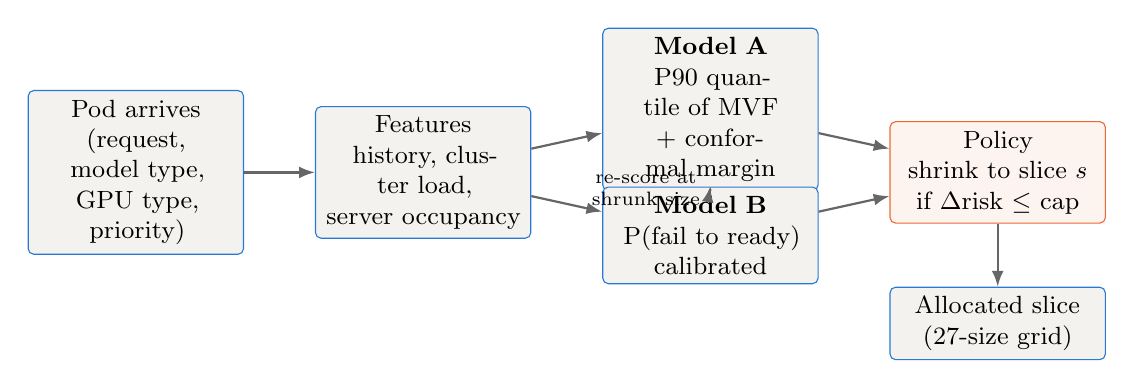
\begin{tikzpicture}[
  node distance=6mm and 9mm,
  box/.style={draw=accent,rounded corners=2pt,fill=soft,align=center,font=\small,minimum height=9mm,text width=2.5cm},
  dec/.style={draw=warn,rounded corners=2pt,fill=warn!8,align=center,font=\small,minimum height=9mm,text width=2.5cm},
  arr/.style={-{Latex[length=2mm]},thick,draw=black!60}]
\node[box] (pod) {Pod arrives\\(request, model type,\\GPU type, priority)};
\node[box,right=of pod] (feat) {Features\\history, cluster load,\\server occupancy};
\node[box,right=of feat,yshift=8mm] (A) {\textbf{Model A}\\P90 quantile of MVF\\+ conformal margin};
\node[box,right=of feat,yshift=-8mm] (B) {\textbf{Model B}\\P(fail to ready)\\calibrated};
\node[dec,right=of A,yshift=-8mm] (pol) {Policy\\shrink to slice $s$\\if $\Delta$risk $\le$ cap};
\node[box,below=8mm of pol] (out) {Allocated slice\\(27-size grid)};
\draw[arr] (pod) -- (feat);
\draw[arr] (feat) -- (A);
\draw[arr] (feat) -- (B);
\draw[arr] (A) -- (pol);
\draw[arr] (B) -- (pol);
\draw[arr] (A.south) to[bend left=10] node[font=\scriptsize,left,align=center]{re-score at\\shrunk size} (B.north);
\draw[arr] (pol) -- (out);
\end{tikzpicture}
\caption{Two-model framing. Model A proposes a smaller slice; Model B re-scores placement risk at that size; the policy accepts the shrink only if the predicted increase in failure risk is under a cap.}
\label{fig:pipeline}
\end{figure}

\subsection{Model families}

\begin{table}[h]
\centering\small
\caption{Model families. Each family received the same tuning budget (three configurations, chosen on validation only).}
\label{tab:models}
\begin{tabularx}{\linewidth}{@{}lL@{}}
\toprule
Model & Description \\
\midrule
A1 & Per-workload 90th percentile of past need over the last 7 days (only pods finished before admission); falls back to the model-type $\times$ GPU-type percentile. \\
A2 & Regularized linear quantile regression ($\tau = 0.90$). \\
A3 & XGBoost quantile regression ($\tau = 0.90$) with monotone constraints on history features. \\
B1 / B2 / B3 & Logistic regression / random forest / LightGBM classifiers for failure to become ready, with Platt or isotonic calibration. \\
\bottomrule
\end{tabularx}
\end{table}

\subsection{Evaluation protocol}
\begin{itemize}
  \item \textbf{Temporal split.} Train days 14--129; validation days 130--157 (split by workload into an early-stopping half and a calibration half); test days 158--183.
  \item \textbf{Leave-one-cluster-out (LOCO).} For each of the 10 clusters with $\ge$9{,}000 pods, train on the other clusters' training days and score that cluster's test days.
  \item \textbf{Safety margin.} Split-conformal margin per (model type $\times$ cold/warm) targeting 95\% coverage, then rounded \emph{up} to one of the 27 slice sizes observed in the trace.
  \item \textbf{Metrics.} Pinball loss ($\tau=0.90$); $U$ = share of pods given less than they needed; $R$ = share of reserved GPU-hours reclaimed; for Model B, PR-AUC, ROC-AUC, Brier, ECE; paired Wilcoxon signed-rank tests across the 10 clusters.
  \item \textbf{Pre-registered gate.} A3 passes only if it beats A1 on pinball loss in $\ge$8 of 10 clusters with Wilcoxon $p \le 0.05$, \emph{and} reclaims more while keeping $U$ near 5\%.
\end{itemize}

% ===========================================================================
\section{Results to Date}
\label{sec:results}

\subsection{Model A: allocation}

\begin{table}[h]
\centering\small
\caption{Model A on unseen clusters (mean of 10 held-out clusters, test days) and on seen clusters (future test days).}
\label{tab:modelA}
\begin{tabular}{@{}lcccc@{\hspace{1.2em}}ccc@{}}
\toprule
& \multicolumn{4}{c}{Unseen clusters (LOCO)} & \multicolumn{3}{c}{Seen clusters} \\
\cmidrule(lr){2-5}\cmidrule(l){6-8}
Model & Pinball & $R$ & $U$ & Coverage & Pinball & $R$ & $U$ \\
\midrule
A1 history rule & \textbf{0.0247} & 11.0\% & \textbf{0.7\%} & \textbf{96.7\%} & 0.0249 & 8.7\% & \textbf{0.5\%} \\
A2 linear QR    & 0.0266 & 12.9\% & 1.4\% & 90.0\% & 0.0266 & 11.1\% & 1.1\% \\
A3 XGBoost QR   & 0.0259 & \textbf{14.3\%} & 2.0\% & 92.2\% & \textbf{0.0237} & \textbf{13.0\%} & 1.0\% \\
\bottomrule
\end{tabular}
\end{table}

\begin{table}[h]
\centering\small
\caption{Pre-registered go/no-go gate for A3 vs.\ A1 on unseen clusters.}
\label{tab:gate}
\begin{tabular}{@{}lll@{}}
\toprule
Criterion & Result & Outcome \\
\midrule
A3 more accurate in $\ge$8 of 10 clusters & 4 of 10 & \textcolor{warn}{\textbf{Fail}} \\
Wilcoxon $p \le 0.05$ on pinball loss & $p = 0.81$ & \textcolor{warn}{\textbf{Fail}} \\
More reclaimed with $U$ near 5\% & 14.3\% vs.\ 11.0\%, $p = 0.007$ & \textcolor{good}{\textbf{Pass}} \\
\midrule
\textbf{Decision} & & \textbf{NO-GO} \\
\bottomrule
\end{tabular}
\end{table}

\paragraph{Matched-risk comparison (exploratory, added after the gate).} Holding every model to exactly $U = 5\%$ in each cluster, A3 is ahead in 8 of 10 clusters by a mean of 1.1 points (median 0.7), reclaiming 21.9\% vs.\ 20.8\% for A1; this is not significant (Wilcoxon $p = 0.14$). The history rule wins clearly in clusters \texttt{3f39} and \texttt{7087}. \Cref{fig:tradeoff} shows the picture: A3's apparent advantage at default margins is mostly bought risk.

\begin{figure}[h]
\centering
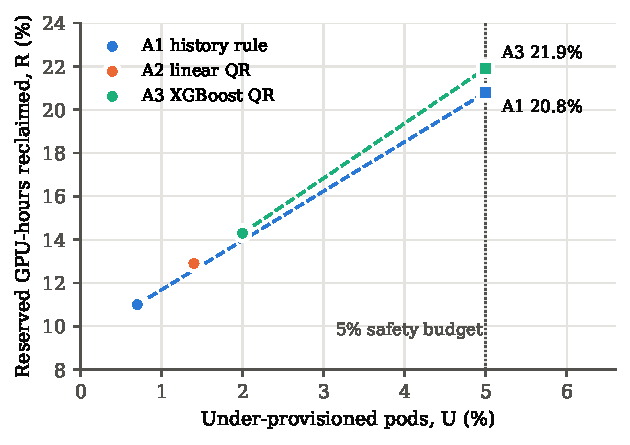
\includegraphics[width=0.62\linewidth]{figures/fig_tradeoff.pdf}
\caption{Reclaim--risk trade-off on unseen clusters. Circles: default conformal margins. Squares: margins re-tuned so each model sits at exactly $U=5\%$. Dashed lines connect the two operating points of the same model and are not measured curves.}
\label{fig:tradeoff}
\end{figure}

\paragraph{Where savings come from.} Almost all reclaimable capacity sits in recommendation pods with workload history (\cref{fig:segments}). A3's one clear advantage is on recommendation pods \emph{without} history (8.1\% vs.\ 0\%), the cold-start case, which motivates the hybrid policy (H10).

\begin{figure}[h]
\centering
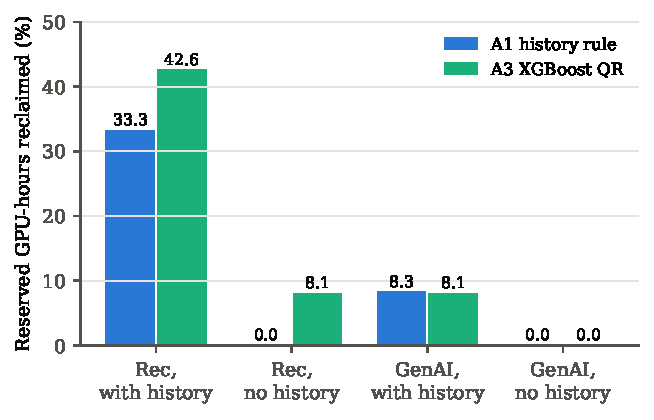
\includegraphics[width=0.62\linewidth]{figures/fig_segments.pdf}
\caption{Reserved GPU-hours reclaimed by pod group (seen clusters, test days).}
\label{fig:segments}
\end{figure}

\paragraph{Other Model A findings.}
\begin{itemize}
  \item \textbf{Slice sizes cap savings.} The 27 sizes in the trace jump from 0.5 to 0.7 to 1.0 GPU, so any pod needing more than 0.7 keeps a whole GPU (\cref{fig:quant}). This alone explains why GenAI pods (median need 0.983) offer almost nothing.
  \item \textbf{Monotone constraints are free.} Removing them changed pinball loss by 0.0000; an audit confirmed no prediction ever decreases as past demand rises.
  \item \textbf{History and cluster load both help.} Removing workload history raised pinball loss by 0.0045 and cut $R$ by 1.4 points; removing cluster-load features pushed $U$ to 4.5\%.
  \item \textbf{Identity features add nothing.} Cluster and switch IDs did not help; separate rec and GenAI models did not beat one pooled model.
  \item \textbf{Sign flips by segment.} \texttt{cpu\_per\_gpu} has Spearman $+0.14$ with need for rec and $-0.47$ for GenAI, so the originally planned $+1$ monotone constraint would have been wrong.
  \item \textbf{Drivers.} Model type and the workload's past maximum need dominate (SHAP and permutation importance); a depth-3 rule tree reproduces A3 with $R^2 = 0.887$.
  \item \textbf{Latency.} A3 scores one pod in 3.6\,ms median, 5.3\,ms p95, well inside an admission-path budget.
\end{itemize}

\begin{figure}[h]
\centering
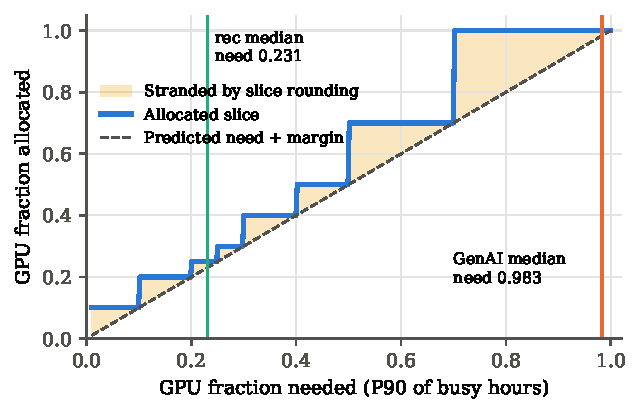
\includegraphics[width=0.58\linewidth]{figures/fig_quantisation.pdf}
\caption{Why the slice grid caps savings. \emph{Illustrative}: the intermediate steps are schematic; the 0.5\ra0.7\ra1.0 jumps and the segment medians are from the trace. Any pod whose need-plus-margin exceeds 0.7 is rounded to a whole GPU.}
\label{fig:quant}
\end{figure}

\subsection{Model B: readiness / failure}

\begin{table}[h]
\centering\small
\caption{Model B discrimination and calibration. Failure base rate 46\% (PR-AUC baseline $\approx$0.46). Seen-cluster ECE is after calibration (B3 uses out-of-fold isotonic); unseen PR-AUC uses raw scores.}
\label{tab:modelB}
\begin{tabular}{@{}lcccccc@{}}
\toprule
& \multicolumn{3}{c}{Seen clusters} & \multicolumn{3}{c}{Unseen clusters} \\
\cmidrule(lr){2-4}\cmidrule(l){5-7}
Model & ROC-AUC & PR-AUC & ECE & ROC-AUC & PR-AUC & ECE \\
\midrule
B1 logistic      & 0.640 & 0.578 & 0.067 & 0.575 & 0.549 & 0.123 \\
B2 random forest & \textbf{0.754} & 0.708 & \textbf{0.044} & \textbf{0.671} & \textbf{0.635} & \textbf{0.112} \\
B3 LightGBM      & \textbf{0.754} & \textbf{0.717} & 0.053 & 0.651 & 0.615 & 0.121 \\
\bottomrule
\end{tabular}
\end{table}

\begin{figure}[h]
\centering
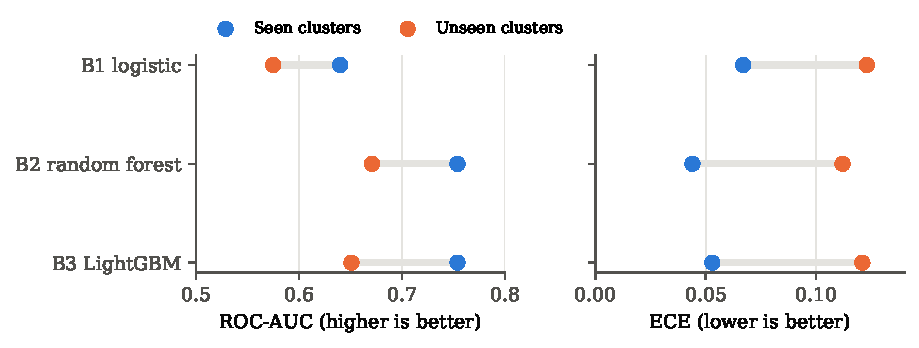
\includegraphics[width=0.85\linewidth]{figures/fig_modelb.pdf}
\caption{Model B transfer gap. Every model loses discrimination and roughly doubles its calibration error on unseen clusters.}
\label{fig:modelb}
\end{figure}

\begin{itemize}
  \item Paired tests over 10 unseen clusters: B3 vs.\ B1 on PR-AUC, better in 6 of 10, $p = 0.065$; on ECE, $p = 0.50$; B3 vs.\ B2, $p = 0.78$. None significant.
  \item \textbf{Why calibration does not transfer:} cluster failure rates range from 35\% to 67\%; a model trained elsewhere cannot know a new cluster's base rate.
  \item Medium risks are underestimated: pods scored at 40\% fail about 50\% of the time.
  \item \textbf{Drivers:} priority class, GPU memory requested, GPU type, past compute use, and server occupancy. Big, low-priority pods asking for scarce GPU types on busy servers fail more often.
  \item \textbf{Latency:} 3.0\,ms median, 7.8\,ms p95.
\end{itemize}

\subsection{Combining A and B}

\begin{table}[h]
\centering\small
\caption{A+B composition on test-day pods requesting $\ge$1 GPU and observed $\ge$24 hours ($n = 55{,}636$).}
\label{tab:compose}
\begin{tabular}{@{}lcccc@{}}
\toprule
\makecell[l]{Risk cap\\per pod} & \makecell{Pods\\shrunk} & \makecell{GPU-hours\\reclaimed} & \makecell{Predicted\\failure risk} & \makecell{Shrunk sizes\\seen in training} \\
\midrule
None      & 27.5\% & 11.4\% & 36.0\% \ra 37.8\% & 12.0\% \\
+10 points & 20.3\% & 7.3\% & 36.0\% \ra 36.5\% & 8.1\% \\
+5 points  & 15.2\% & 5.3\% & 36.0\% \ra 36.1\% & 5.5\% \\
+2 points  & 10.5\% & 3.4\% & 36.0\% \ra 35.9\% & 3.6\% \\
\bottomrule
\end{tabular}
\end{table}

\begin{figure}[h]
\centering
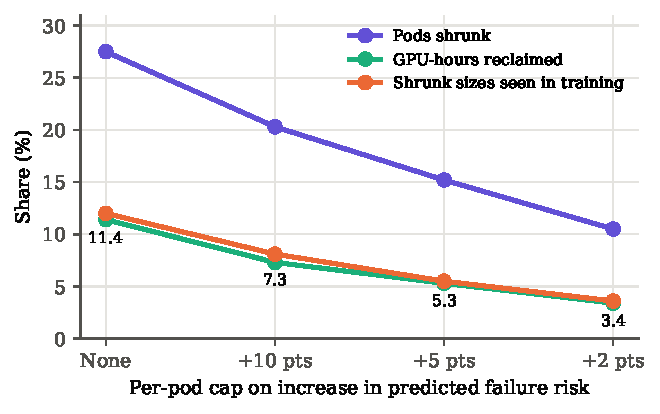
\includegraphics[width=0.6\linewidth]{figures/fig_composition.pdf}
\caption{The tighter the risk cap, the fewer shrunk pods land on a slice size Model B has ever observed. Under the +2-point cap only 3.6\% do, so the ``safe'' shrinks are mostly extrapolation.}
\label{fig:compose}
\end{figure}

Shrinking pods with Model A and re-scoring them with Model B reclaims 11.4\% of long-running pods' GPU-hours, but fractional-GPU pods make up only 0.3--3.7\% of each cluster, consistent with the OSDI~'26 finding that GPU sharing is rarely used. The composition is therefore reported as a \emph{what-if}, not a validated policy.

\subsection{Answers so far}

\begin{table}[h]
\centering\small
\caption{Answers to the pre-registered research questions.}
\label{tab:answers}
\begin{tabularx}{\linewidth}{@{}p{4.4cm}L@{}}
\toprule
Question & Answer \\
\midrule
RQ1: Can the minimum viable slice be predicted better than the percentile-over-history heuristic? & \textbf{No} on unseen clusters: A3 better in 4 of 10, $p = 0.81$ (NO-GO). At matched 5\% risk, 21.9\% vs.\ 20.8\% reclaimed, $p = 0.14$. \\
RQ2: Is failure to become ready predictable and calibrated? & \textbf{Yes} within known clusters (ROC-AUC 0.75, ECE 0.05); weaker and miscalibrated on unseen clusters (ROC-AUC 0.65, ECE 0.12). \\
RQ3: How much reserved capacity is reclaimable at a fixed risk? & About \textbf{21\%} of reserved GPU-hours at $U = 5\%$ in the D1 population, almost all from recommendation pods with history. The placement-risk side cannot yet be estimated reliably. \\
RQ4: Do relationships transfer to unseen clusters? & \textbf{Partly}: accuracy roughly holds, but conformal coverage falls to 92\% (target 95\%) and Model B's probabilities do not transfer. \\
\bottomrule
\end{tabularx}
\end{table}

% ===========================================================================
\section{Failures, Negative Results, and What They Taught Us}
\label{sec:failures}

Negative results are kept in full here because they are the most transferable part of the work.

\begin{longtable}{@{}p{3.4cm}p{5.6cm}p{5.6cm}@{}}
\caption{Failure log.}\label{tab:failures}\\
\toprule
What failed & Evidence & Lesson / response \\
\midrule
\endfirsthead
\toprule
What failed & Evidence & Lesson / response \\
\midrule
\endhead
Learned model vs.\ history rule (H1) & A3 better in 4/10 unseen clusters, $p=0.81$; gate NO-GO. & Inference demand is dominated by per-workload persistence. A simple rule is the right production baseline; ML earns its keep only where history is missing (cold start). \\
Early research question & First framing (``increase utilization without compromising SLA'') had no latency field to measure SLA against. & Reframed around $U$ (under-provisioning rate) as an observable safety proxy; latency stays a stated limitation. \\
Missing timestamps & Day/hour fields absent on ingest. & Recovered from file paths; added a data-validation step before any split. \\
History-feature leakage & Building \texttt{wl\_hist\_*} from pods \emph{admitted} on earlier days gave 8\% lower test error than using only pods \emph{finished} before admission. & Exported history columns probably carry future information. Rebuild in SQL with a strict finished-before-admission cut (\cref{sec:experiments}, E9). \\
Planned monotone constraint on \texttt{cpu\_per\_gpu} & Spearman $+0.14$ (rec) vs.\ $-0.47$ (GenAI). & Domain priors must be checked per segment before they become constraints. \\
Segment-specific models & Separate rec/GenAI models did not beat a pooled model. & Model type is already a dominant split feature; pooling is simpler and as good. \\
Cluster/switch ID features & No gain. & Identity features do not generalize; use cluster \emph{state} (load, occupancy) instead. \\
Model B calibration transfer & ECE 0.04--0.07 seen \ra 0.11--0.12 unseen; base rates 35--67\% by cluster. & Needs per-cluster base-rate recalibration (E8) or a hierarchical prior. \\
Boosting vs.\ random forest for B & B3 vs.\ B2 $p=0.78$. & Model class is not the bottleneck; features and support are. \\
A+B composition & Only 3.6--12\% of shrunk sizes appear in training. & Model B cannot score counterfactual sizes it never saw. Needs either more fractional-GPU data or a simulator (Tier 3). \\
Conformal coverage on unseen clusters & 92.2\% vs.\ 95\% target for A3. & Exchangeability breaks across clusters; per-cluster or weighted conformal is needed. \\
\bottomrule
\end{longtable}

% ===========================================================================
\section{Our Setting vs.\ Industry: Why the Results Differ}
\label{sec:comparison}

\begin{table}[h]
\centering\small
\caption{Side-by-side comparison of a production scheduler's vantage point with what the ASI trace exposes to this project.}
\label{tab:compare}
\begin{tabularx}{\linewidth}{@{}P{2.6cm}LL@{}}
\toprule
Dimension & Production schedulers (Google, AWS, Azure, Meta, Alibaba internal) & This project (ASI public trace) \\
\midrule
Available features & Live per-request latency, queue depth, model identity, kernel profiles, traffic forecasts, load-test results & Requests, priority, GPU type, model type (anonymized), 20-s utilization telemetry, server/switch topology. \textbf{No request latency.} \\
Workload granularity & Per request / token (Aegaeon, Dynamo), per kernel (Orion, REEF), per container & Per pod, labelled by hourly-P90 busy-hour demand \\
Allocation granularity & MIG profiles, MPS percentages, time-slices, live resize & 27 slice sizes as observed; 0.5\ra0.7\ra1.0 jumps; fractional pods only 0.3--3.7\% per cluster \\
Compute scale & 10$^4$--10$^5$+ GPUs, continuous & Up to 155{,}410 GPUs, but a 294k-pod (A) / 2.8M-pod (B) modelling slice; 10 LOCO clusters \\
Scheduler constraints & Isolation, gang scheduling, topology, GPU-model pinning, preemption policy & Same constraints are \emph{in} the data but not controllable; $>$99\% of jobs pin a GPU model \\
Production requirements & Hard SLOs, A/B rollout, fault isolation, rollback & Safety proxy $U \le 5\%$; readiness failure as placement risk \\
Actuation & Scheduler can act and observe the consequence & Observational only: no counterfactual sizes \\
\bottomrule
\end{tabularx}
\end{table}

\subsection{Why our numbers differ, and why that is informative}

\begin{enumerate}
  \item \textbf{We measure opportunity; industry reports realized savings.} Autopilot's 46--60\%\ra23\% slack reduction and SpotGPU's 68\%\ra93\% allocation are outcomes of systems that can act. Our 21--25\% is an \emph{upper bound on reclaimable reservation} at a stated risk, before packing and actuation losses. The two answer different questions and should not be ranked against each other.
  \item \textbf{Different lever, same headroom.} SpotGPU harvests reserved-but-idle capacity \emph{after} reservation by lending it to preemptible jobs; our Model A shrinks the reservation \emph{at admission}. They target the same idle headroom from opposite ends, so our number partly overlaps SpotGPU's gain. This positions right-sizing as complementary (it reduces how much must be harvested and evicted) rather than as a competitor.
  \item \textbf{The slice grid, not the predictor, is the binding constraint.} Industry gets finer control (MIG sevenths, MPS percentages, token-level switching). In ASI, sharing is rare because isolation is weak, so the trace contains almost no fractional allocations to learn from. This explains both the GenAI zero and Model B's extrapolation in \cref{tab:compose}.
  \item \textbf{GenAI is memory-bound, not compute-bound.} ASI reports GenAI online inference at 94\% GPU memory but 5\% SM. Our median GenAI MVF of 0.983 is consistent with a \emph{memory-dominated} label. A GenAI pod cannot be shrunk by memory, but its idle SMs are exactly what a compute-light recommendation pod could use. This turns the GenAI ``zero'' into the motivation for the workload-mixing experiment (E1) rather than a dead end. \emph{To verify: which resource term dominates our MVF label per segment.}
  \item \textbf{Simple rules win when demand is persistent.} Autopilot's production recommender is itself a decayed percentile with a margin, essentially our A1. Our NO-GO result matches industry practice: learned models add most where history is missing.
  \item \textbf{Generalization is tested harder here.} Industry models are retrained per cluster continuously; we test on clusters never seen in training. The calibration drop for Model B (ECE 0.05\ra0.12) is the price of that stricter test, and it quantifies how much per-cluster recalibration (E8) is worth.
\end{enumerate}

\subsection{Which gaps are addressable, and which are inherent?}

\begin{table}[h]
\centering\small
\caption{Gap taxonomy. \emph{Modelling} and \emph{feature engineering} gaps can be closed within this project; \emph{inherent} gaps are properties of a public, anonymized, observational trace and are reported, not fixed.}
\label{tab:gaps}
\begin{tabularx}{\linewidth}{@{}P{3.2cm}P{1.9cm}LP{1.0cm}@{}}
\toprule
Gap vs.\ industry & Type & What we can do & Exp. \\
\midrule
Leaky history features & Modelling & Strict finished-before-admission rebuild. & E9 \\
Hourly-P90 labels miss peaks & Modelling & P99/max labels from 20-s telemetry; separate memory (hard) and compute (soft). & E9, E5 \\
Calibration does not transfer & Modelling & Prior-shift recalibration; weighted conformal. & E8 \\
Uniform 5\% safety budget & Modelling & Segment- and priority-aware budgets. & E5 \\
Cold-start pods (61--68\%) & Feature eng. & Early-runtime features; resize after warm-up; hybrid routing. & E4, E6 \\
No co-location / interference signal & Feature eng. & Server/ASW workload-mix features; segregate vs.\ interleave what-if. & E1 \\
Hardware heterogeneity & Feature eng. & Compatibility cells; throughput-normalized need. & E2 \\
Production tiers & Feature eng. & Priority-class segmentation and interactions. & E3 \\
\midrule
Coarse 27-size slice grid & Inherent (boundable) & What-if re-rounding gives an upper bound only. & E7 \\
No request latency / SLO field & Inherent & Use $U$ as proxy; state clearly that SLA neutrality is not shown. & -- \\
No counterfactual placements & Inherent (partly) & Simulator replay; flag A+B results as what-if. & E10 \\
No actuation (cannot resize live) & Inherent & Estimate opportunity, not realized savings. & -- \\
Anonymized model identities & Inherent & Use model-type and workload IDs only. & -- \\
One operator, six months & Inherent & LOCO across 10 clusters; Tier-2 transfer if time permits. & E10 \\
\bottomrule
\end{tabularx}
\end{table}



% ===========================================================================
\section{Business Value}
\label{sec:value}

\subsection{Framing the headline number}
The current result is that \textbf{about 21--25\% of reserved online-inference GPU-hours} are reclaimable while keeping under-provisioning at or below the \textbf{5\% safety constraint} ($U \le 5\%$). The 21\% end is the measured matched-risk result on unseen clusters (20.8\% A1, 21.9\% A3); the 25\% end is the upper end of the current estimate range and should be treated as provisional until E9 removes the history-feature leakage. Three tiers keep the claim honest:

\begin{table}[h]
\centering\small
\caption{Savings tiers, from opportunity to risk-constrained policy.}
\label{tab:tiers}
\begin{tabularx}{\linewidth}{@{}p{3.3cm}cL@{}}
\toprule
Tier & Reclaimed & What it assumes \\
\midrule
Opportunity (upper) & 25\% & Provisional upper estimate; Model A only; perfect packing of freed slices. \\
Opportunity (measured) & 21\% & Matched $U=5\%$ on unseen clusters; Model A only; perfect packing. \\
A+B policy, no risk cap & 11.4\% & Long-running pods; Model B re-scores each shrink; risk rises 36.0\%\ra37.8\%. \\
A+B policy, +2-point cap & 3.4\% & Only shrinks Model B deems near-risk-neutral; mostly extrapolated sizes. \\
\bottomrule
\end{tabularx}
\end{table}

\subsection{Lower GPU cost}
Per 1{,}000 reserved GPUs there are $1{,}000 \times 8{,}760 = 8.76$M GPU-hours per year. Reclaiming a share $r$ frees $r \times 8.76$M GPU-hours, or equivalently $r \times 1{,}000$ GPUs of steady capacity. We price this at three illustrative on-demand rates: $\approx$\$1/GPU-h for A10-class cards (approximate; ASI's online fleet is dominated by A10, L20 and H20 parts), \$3.43 for A100 80GB (AWS p4de per GPU), and \$3.90 for H100 (AWS P5 after the June 2025 price cut~\cite{aws2025price}, from secondary aggregators). Owned fleets have lower effective rates than on-demand, so these are upper-range translations.

\begin{table}[h]
\centering\small
\caption{Annual value per 1{,}000 reserved inference GPUs. GPU-hours in millions; dollars in millions per year. Scale linearly with fleet size.}
\label{tab:value}
\begin{tabular}{@{}lcccccc@{}}
\toprule
Tier & Reclaimed & GPU-h freed & GPUs freed & @\$1.00 & @\$3.43 & @\$3.90 \\
\midrule
Opportunity (upper) & 25\% & 2.19 & 250 & \$2.19 & \$7.51 & \$8.54 \\
Opportunity (measured) & 21\% & 1.84 & 210 & \$1.84 & \$6.31 & \$7.17 \\
A+B, no cap & 11.4\% & 1.00 & 114 & \$1.00 & \$3.43 & \$3.89 \\
A+B, +2-pt cap & 3.4\% & 0.30 & 34 & \$0.30 & \$1.02 & \$1.16 \\
\bottomrule
\end{tabular}
\end{table}

\begin{figure}[h]
\centering
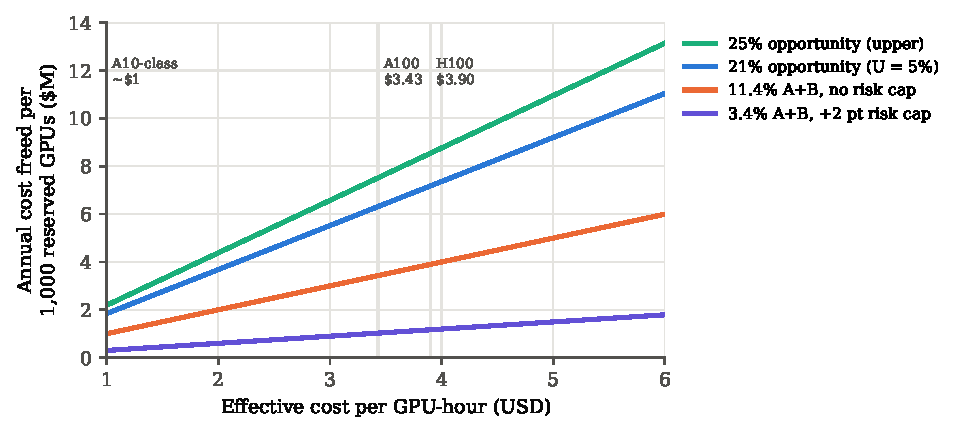
\includegraphics[width=0.8\linewidth]{figures/fig_value.pdf}
\caption{Annual cost freed per 1{,}000 reserved GPUs as a function of effective GPU-hour price, for each savings tier.}
\label{fig:value}
\end{figure}

\noindent For capital planning, \cref{eq:util} gives the same story: reclaiming 21\% of reservations is equivalent to raising effective utilization of the reserved pool by a factor of $1/(1-0.21) \approx 1.27$, so a fleet sized for today's demand could absorb $\approx$27\% more of the same workload before buying GPUs.

\subsection{Less idle capacity}
ASI reports online-inference median SM utilization of 6\% and an allocation ratio of 68\% for high-priority work before SpotGPU~\cite{li2026asi}. Right-sizing at admission shrinks reservations \emph{before} they become idle headroom. Because recommendation pods hold most of the reclaimable capacity (33--43\% for rec-with-history), the most direct win is consolidating recommendation serving onto fewer GPUs.

\subsection{Faster job completion}
Capacity freed from over-reserved inference does not disappear; it returns to the pool used by preemptible training, offline inference and development jobs. In ASI, low-priority jobs already run on harvested capacity, and making that capacity \emph{reserved-free} rather than \emph{borrowed} reduces evictions; ASI's preemption-cost-aware victim selection alone cut low-priority completion time by 24\%~\cite{li2026asi}. We do not estimate a JCT gain from the trace; the simulator (E10) would.

\subsection{More reliable provisioning}
Model B addresses a separate cost: 46\% of D2 pods fail to become ready, and each failed placement temporarily occupies GPUs. Zhang and Liao~\cite{zhang2026ineffective} show readiness-aware ordering cuts ineffective occupancy from 43.64\% to 27.15\% on an Alibaba trace. A calibrated Model B used as a veto keeps right-sizing from trading GPU-hours for failed placements, and used on its own could steer risky pods (large, low-priority, scarce GPU type, busy server) to safer placements.

\subsection{Caveats on value}
Realized savings will be lower than the opportunity tiers because (i) freed fractions must be packable onto shared GPUs, and ASI shows sharing is rare due to weak isolation; (ii) $U$ is not a latency SLO; (iii) the A+B tiers rely on Model B extrapolating to unseen sizes. The value table should be read as the ceiling that justifies building the mechanism, not as a forecast.


% ===========================================================================
\section{Proposed Experiments and Feature Engineering}
\label{sec:experiments}

Every experiment below is \status{proposed}: designed, with a hypothesis and a decision rule fixed in advance, but not yet run. All keep the same splits, LOCO protocol, conformal margins and metrics as \cref{sec:method}, so results remain comparable to \cref{tab:modelA,tab:modelB}. Each is tagged by the model it informs: \textbf{A} (allocation), \textbf{B} (readiness/failure), or \textbf{A+B} (policy).

\subsection{New feature families}

\begin{table}[h]
\centering\small
\caption{Candidate features. All are computed strictly from information available at admission time $t_0$ (or at $t_0 + k$ hours for E4).}
\label{tab:features}
\begin{tabularx}{\linewidth}{@{}P{2.5cm}LP{0.9cm}P{1.1cm}@{}}
\toprule
Family & Definition (at admission) & Model & Exp. \\
\midrule
Server workload mix & Share of the target server's allocated GPUs held by rec / GenAI / training / offline-inference / dev pods; Shannon entropy of that mix; count of distinct workload types. & A, B & E1 \\
Switch (ASW) mix & Same shares aggregated over the access switch; captures network and host contention beyond one server. & A, B & E1 \\
Same-type co-tenancy & Number of pods of the \emph{same workload} already on the server (replica spreading vs.\ stacking). & B & E1 \\
Compatibility & Requested GPU memory $/$ GPU-type memory capacity; GPU-type scarcity = free GPUs of that type in the cluster $/$ requests pending; historical failure rate of (model type $\times$ GPU type $\times$ slice) cell, hierarchically smoothed. & B (A) & E2 \\
Normalized need & MVF rescaled by GPU-type throughput so need is comparable across generations. & A & E2 \\
Priority / production & Priority class (production vs.\ best-effort / spot); preemptible flag; tenant's share of high-priority pods. & A, B & E3 \\
Runtime shape & From the first $k$ hours of telemetry: peak-to-mean ratio, coefficient of variation, 24-h autocorrelation (diurnal strength), slope. & A & E4 \\
Memory headroom & Max / P99 of GPU-memory use (vs.\ P90 of utilization) to separate hard (OOM) from soft (slowdown) constraints. & A & E5, E9 \\
\bottomrule
\end{tabularx}
\end{table}

\subsection{Experiment cards}

\newcommand{\expcard}[7]{%
\begin{tcolorbox}[colback=white,colframe=black!25,boxrule=0.5pt,arc=2pt,left=5pt,right=5pt,top=3pt,bottom=3pt,title={\small\textbf{#1}\hfill\textsc{#2}},colbacktitle=soft,coltitle=black,fonttitle=\small]
\small
\textbf{Hypothesis.} #3\par\smallskip
\textbf{Design.} #4\par\smallskip
\textbf{Metric \& decision rule.} #5\par\smallskip
\textbf{Why it matters.} #6\par\smallskip
\textbf{Feasibility.} #7
\end{tcolorbox}}

\expcard{E1. Workload mixing: recommendation grouped vs.\ mixed with GenAI}{A, B}
{(H5) Rec pods admitted to servers whose GPUs are predominantly held by other rec pods have lower and more predictable MVF than rec pods co-located with GenAI or training. Co-location features reduce A's pinball loss and raise B's PR-AUC.}
{(i) Stratify D1 rec pods into \emph{rec-homogeneous} ($\ge$80\% of the server's allocated GPUs are rec), \emph{GenAI-mixed} ($\ge$20\% GenAI), and \emph{other-mixed}. Compare MVF distributions, within-workload variance, and A1 pinball loss by stratum. (ii) Add the server/ASW mix features of \cref{tab:features} to A3 and B3; ablate. (iii) Packing what-if: bin-pack each test day's predicted slices under two placement rules (\emph{segregate}: rec with rec, GenAI with GenAI; \emph{interleave}: first-fit across both) and count GPUs freed.}
{Mix features are kept if they improve pinball loss in $\ge$7 of 10 LOCO clusters (Wilcoxon $p\le0.05$) without raising $U$, or improve B's PR-AUC by $\ge$0.02. The packing what-if is reported as an upper bound.}
{Industry schedulers co-locate latency-critical and best-effort work deliberately (\cref{sec:industry}). If mixing raises variance, segregation is a free policy lever; if it does not, operators can interleave and pack tighter.}
{Addressable with the trace's per-server allocation tables. Caveat: in ASI most pods hold whole GPUs, so ``mixing'' is mostly \emph{host-level} (CPU, PCIe, NIC) rather than SM-level sharing. The result says nothing about true MPS/MIG interference.}

\expcard{E2. Workload--pod--GPU compatibility}{B (A)}
{(H6) Readiness failure is driven by the interaction (workload type $\times$ GPU type $\times$ requested size), especially requests for scarce GPU types, more than by any main effect. GPU-normalized need makes MVF transfer better across clusters with different hardware mixes.}
{Build a compatibility matrix of failure rate by cell with empirical-Bayes smoothing; add cell rate, memory-fit ratio and scarcity to B; add throughput-normalized need as an alternative A target.}
{B: unseen-cluster PR-AUC and ECE vs.\ \cref{tab:modelB}. A: unseen-cluster coverage closer to 95\% than 92.2\%.}
{Mirrors how commercial schedulers filter by node affinity, GPU product labels and MIG profiles before scoring.}
{Addressable. Risk: sparse cells; smoothing and a minimum-count rule are mandatory.}

\expcard{E3. Production vs.\ non-production behaviour}{A, B}
{(H7) Production (high-priority) pods have tighter, more persistent demand, lower failure, and a smaller reclaimable share; low-priority pods fail more when placed on servers with many production pods.}
{Segment by priority class. Report MVF median/IQR, A1 vs.\ A3 reclaim at $U=5\%$, and B failure rate per segment. Fit per-segment conformal margins. Interaction test for (pod priority $\times$ server production share) in B.}
{Report per-segment $R$ at matched $U$; the interaction is kept if its permutation importance is in B's top 10 on unseen clusters.}
{Production requirements differ: a GenAI chat endpoint and a best-effort batch scorer should not carry the same safety budget (feeds E5).}
{Addressable: priority classes are in the trace. Limitation: priority is a proxy for ``production''; no explicit SLO tier.}

\expcard{E4. Runtime patterns and a second decision point}{A}
{(H8) For cold-start pods (61--68\% of the population), the first $k\in\{1,6,24\}$ hours of telemetry predict MVF far better than admission-time features, so a \emph{resize-after-warm-up} policy reclaims more than admission-time sizing.}
{Add runtime-shape features (\cref{tab:features}) computed on $[t_0, t_0+k]$; predict MVF over the remaining lifetime. Compare reclaim at $U=5\%$ for admission-only vs.\ $k$-hour resize, charging the first $k$ hours at the original size.}
{Net GPU-hours reclaimed vs.\ admission-only A3, by $k$.}
{This is how vertical autoscalers in industry work (observe, then resize). It directly attacks the cold-start gap where A3 is the only thing that helps.}
{Addressable from 20-s telemetry. Assumes in-place resize or cheap restart; ASI's actual mechanism is unknown.}

\expcard{E5. Explicit, segment-aware safety constraints}{A+B}
{(H9) A per-segment risk budget (e.g.\ 1--2\% for GenAI/production, 5--8\% for rec/non-production) reclaims more GPU-hours than a uniform 5\% at equal or lower \emph{expected harm}, where harm weights an under-provisioned production pod higher. GPU memory must be treated as a hard constraint (max/P99) and compute as a soft one (P90).}
{Define harm $H=\sum_s w_s U_s n_s$ with $w_s$ set by priority. Solve for per-segment margins that maximize $R$ subject to $H \le H_{\text{uniform 5\%}}$. Separate memory and compute quantile targets.}
{$R$ at matched $H$; also report worst-cluster $U$ to show tail safety.}
{Translates ``5\% safety constraint'' into an operator-facing knob tied to business priority.}
{Addressable. Harm weights are an assumption; report a sensitivity sweep.}

\expcard{E6. Hybrid policy}{A}
{(H10) Using A1 for warm pods and A3 for cold-start pods matches A1 where it is strong and adds A3's 8.1-point gain on rec-no-history.}
{Route by history availability; same LOCO protocol.}
{$R$ at $U=5\%$ vs.\ both parents; Wilcoxon over clusters.}
{Deployable, interpretable, and consistent with the NO-GO finding.}
{Addressable immediately.}

\expcard{E7. Finer slice sizes (what-if)}{A}
{Adding sizes between 0.5 and 1.0 GPU (e.g.\ MIG-like sevenths, or 0.6/0.75/0.8/0.9) unlocks GenAI and large-rec reclaim currently blocked by rounding (\cref{fig:quant}).}
{Re-round A1/A3 predictions to alternative grids; recompute $R$, $U$.}
{Reclaim by grid; marginal gain per added size.}
{Quantifies the value of hardware partitioning (MIG profiles) vs.\ better prediction.}
{Upper bound only: assumes the slice is actually enforceable and isolated.}

\expcard{E8. Per-cluster recalibration}{A, B}
{Most of B's unseen-cluster calibration error is base-rate shift (35--67\% failure by cluster), so a prior-shift correction from a small labelled sample (first day) restores ECE $\le$0.06; weighted conformal restores A's coverage to $\approx$95\%.}
{Label-shift adjustment of B's logits using day-1 base rate; covariate-weighted split conformal for A. Robustness check: replicate Zhang and Liao's machine-grouped 5-fold protocol~\cite{zhang2026ineffective} on D2 to show how much of the AUC gap (0.82 vs.\ 0.65--0.75) is due to evaluation protocol.}
{Unseen-cluster ECE and coverage before/after.}
{Commercial systems recalibrate per region/cluster continuously; this is the cheapest fix for the transfer gap.}
{Addressable.}

\expcard{E9. Leakage-free history and peak-aware labels}{A}
{Rebuilding \texttt{wl\_hist\_*} from pods \emph{finished} before admission removes the 8\% optimistic bias; P99/max memory labels raise required slices modestly but make $U$ meaningful.}
{SQL rebuild; re-run the full gate on fixed data before any other experiment is trusted.}
{Change in pinball, $R$, $U$ vs.\ \cref{tab:modelA}.}
{Every other result depends on this.}
{Addressable; highest priority.}

\expcard{E10. Stretch: transfer and simulation}{A+B}
{Findings transfer to a second trace (Tier 2, xMaaS) and survive a scheduler replay (Tier 3) where shrunk pods are actually placed.}
{Replay the test window in a simple discrete-event simulator with predicted slices; measure placement failures, queueing delay and GPUs freed.}
{Simulated $R$ vs.\ trace-estimated $R$.}
{Closes the counterfactual gap that Model B cannot.}
{Partly addressable; simulator fidelity is the main threat.}

\subsection{Experiment summary}

\begin{table}[h]
\centering\small
\caption{Experiments by priority. Gap type refers to \cref{tab:gaps}.}
\label{tab:expsummary}
\begin{tabular}{@{}llllc@{}}
\toprule
ID & Topic & Model & Gap type & Priority \\
\midrule
E9 & Leakage-free history, P99 labels & A & Modelling & 1 \\
E6 & Hybrid policy & A & Modelling & 1 \\
E1 & Workload mixing (rec vs.\ GenAI) & A, B & Feature eng. & 2 \\
E2 & Workload--GPU compatibility & B & Feature eng. & 2 \\
E3 & Production vs.\ non-production & A, B & Feature eng. & 2 \\
E4 & Runtime patterns / resize & A & Feature eng. & 2 \\
E8 & Per-cluster recalibration & A, B & Modelling & 2 \\
E5 & Segment-aware safety budgets & A+B & Modelling & 3 \\
E7 & Finer slices (what-if) & A & Inherent (bounded) & 3 \\
E10 & Transfer + simulator & A+B & Inherent (partly) & stretch \\
\bottomrule
\end{tabular}
\end{table}


% ===========================================================================
\section{Limitations}
\label{sec:limitations}

\begin{itemize}
  \item \textbf{No latency data.} $U$ is the only safety proxy; the trace has no request-latency or SLO-violation field. We cannot claim SLA neutrality, only that predicted slices cover observed busy-hour demand.
  \item \textbf{Labels are P90s of hourly averages.} Telemetry is sampled every 20 seconds, so true peaks are higher. The GPU-memory term should use a maximum or P99.
  \item \textbf{Possible leakage} in history features (\cref{tab:failures}).
  \item \textbf{Reclaiming needs a mechanism.} The operator reports GPU sharing is rarely used because isolation is weak, and its own SpotGPU mechanism already raises allocation from 68\% to 93\%. How reclaimed slices would be consumed is open.
  \item \textbf{Counterfactual blindness.} The trace records what was allocated, not what would have happened at a smaller size; Model B extrapolates.
  \item \textbf{External validity.} One operator, one six-month window, 10 usable held-out clusters; anonymized model identities.
\end{itemize}

% ===========================================================================
\section{Plan and Timeline}
\label{sec:timeline}

Phases 0--5 of the original plan (data, datasets, baselines, Model A, Model B, composition) are complete; interpretation is done for Model A. \Cref{fig:gantt} lays out the remaining work.

\begin{figure}[h]
\centering
\resizebox{\linewidth}{!}{%
\begin{ganttchart}[
  hgrid, vgrid={*1{dotted}},
  x unit=1.0cm, y unit chart=0.55cm,
  title height=1,
  bar/.append style={fill=accent!70,draw=accent},
  milestone/.append style={fill=warn,draw=warn},
  group/.append style={fill=black!60},
  bar label font=\small, group label font=\small\bfseries,
  milestone label font=\small\itshape
]{1}{8}
\gantttitle{Weeks from Oct 26, 2026}{8} \\
\gantttitlelist{1,...,8}{1} \\
\ganttgroup{Fix foundations}{1}{2} \\
\ganttbar{E9 leakage-free history; P99 labels}{1}{2} \\
\ganttbar{Re-run A1/A3 gate on fixed data}{2}{2} \\
\ganttgroup{New signals}{2}{5} \\
\ganttbar{E1 workload-mixing features}{2}{4} \\
\ganttbar{E2 compatibility; E3 prod/non-prod}{3}{4} \\
\ganttbar{E4 runtime patterns (cold start)}{4}{5} \\
\ganttgroup{Policies}{5}{6} \\
\ganttbar{E5 per-segment safety; E6 hybrid; E7 slices}{5}{6} \\
\ganttbar{E8 per-cluster recalibration}{5}{6} \\
\ganttmilestone{Results freeze}{6} \\
\ganttgroup{Write-up}{7}{8} \\
\ganttbar{Compress to page limit; final report}{7}{8} \\
\ganttbar{Stretch: Tier 2/3 transfer \& simulator}{7}{8}
\end{ganttchart}}
\caption{Remaining work. Stretch items are cut first if time runs short.}
\label{fig:gantt}
\end{figure}

% ===========================================================================
\section{Conclusion}
\label{sec:conclusion}

The headline is a useful negative result wrapped around a positive one. \emph{Positive:} at a 5\% under-provisioning budget, roughly a fifth to a quarter of reserved online-inference GPU-hours are reclaimable on clusters never seen in training, concentrated in recommendation pods with history. \emph{Negative:} a learned model does not beat a per-workload history rule on accuracy; most of the value is reachable with a rule an operator could deploy this week, and ML's marginal value is confined to cold-start pods. \emph{Open:} the placement-risk side, because the trace barely contains the fractional allocations a right-sizing policy would create.

Compared to commercial schedulers, this gap is expected rather than embarrassing: production systems own the actuation path (MIG, MPS, time-slicing, live resize), observe latency, and can run controlled experiments, while a trace-based study can only estimate the \emph{opportunity}. The next round of work targets the gaps that modelling can close (leakage, labels, workload-mixing and runtime features, per-cluster calibration, segment-specific safety budgets) and documents honestly the ones it cannot.

\bibliographystyle{plainnat}
\bibliography{refs}

% ===========================================================================
\appendix
\section{Research Trail (Chronological)}
\label{app:trail}

\begin{table}[H]
\centering\small
\begin{tabularx}{\linewidth}{@{}p{2.4cm}L@{}}
\toprule
When & Step \\
\midrule
Early Sep 2026 & Topic chosen: can GPU-trace patterns raise utilization without compromising inference latency/SLA? Motivation via utilization identity (\cref{eq:util}). Dataset: ASI trace. Open items: schema, sampling, scope, compute budget. \\
Mid Sep 2026 & 1--2\% sample used for first visualizations. Scope narrowed to rec + GenAI online inference (supervisor comment). References gathered: OSDI~'26 ASI, Philly traces, Resource Central. \\
Late Sep 2026 & Day/hour recovery; D1 and D2 built; plan pre-registered (models, splits, LOCO, conformal, go/no-go gate). \\
Oct 4, 2026 & Progress report: Phases 0--5 done. Model A NO-GO on accuracy gate; $\approx$21\% reclaimable at $U=5\%$; Model B AUC 0.75/0.65; A+B composition as what-if. \\
Oct 26, 2026 & Reference audit: the OSDI~'26 PDF link in the early notes (\texttt{osdi26-wu-tianyuan.pdf}) is the WEAVE RL post-training paper; the ASI trace paper is Li et al.~\cite{li2026asi}. Closest prior work to Model B found~\cite{zhang2026ineffective}. \\
Oct 26, 2026 & This proposal: industry comparison, gap taxonomy, business value, next experiments (E1--E10). \\
\bottomrule
\end{tabularx}
\end{table}

\section{Reproducibility}
All figures are regenerated by \texttt{scripts/make\_figures.py} from the numbers reported in \cref{sec:results}; no figure in this document reports a \status{proposed} experiment. The proposal compiles with \texttt{tectonic main.tex}.

\end{document}
